\newpage
\section{Auswertung}
\label{sec:Auswertung}



\subsection{Bestimmung der Metalle über die Dichte}
Die Metalle lassen sich über ihr Volumen V und ihre Masse m bestimmen(Tab.1).
Im Vergleich zu dem Literaturwert von Messing mit $8.41\, \frac{g}{cm^3}$\cite{litval}
zeigt sich, dass beide Stäbe aus Messing bestehen.
\begin{table}[h]
  \centering
  \label{tab:2}
  \begin{tabular}{ c c c c c c }
    \toprule
    {$\text{Stab}$}
   &{$l \,\, \text{in} \, [cm]$}
   &{$d \,\, \text{in} \, [cm]$}
   %&{$h \, in \, [m]$}
   &{$V \,\, \text{in} \, [cm^3]$}
   &{$m \,\, \text{in} \, [g]$}
   &{$\rho \,\, \text{in} \, [\frac{g}{cm^3}]$} \\
    \midrule
     {$\text{eckig}$}&60&1&60&502.4 & 8.367 \\
     {$\text{rund}$}&60.05&1&15$\pi$&394.4 & 8.361 \\
    \bottomrule
  \end{tabular}
  \caption{Dichte der Metalle}
\end{table}


\subsection{Eckiger Stab, einseitige Einspannung}

\begin{table}[h]
  \centering
  \label{tab:3}
  \begin{tabular}{ c c }
    \toprule
    $x \,\, \text{in} \, [mm]$
   &{$D(x) \,\, \text{in} \, [mm]$}\\
   %&{$(Lx^2- \frac{x^3}{3}) \,\, \text{in} \, [10^{-3}m^3]$} \\

    \midrule
    30  & 0.065\\% 0.43\\
    50  & 0.135\\% 1.19\\
    70  & 0.225\\% 2.30\\
    90  & 0.390\\% 3.75\\
    110 & 0.530\\% 5.52\\
    130 & 0.670\\% 7.60\\
    150 & 0.875\\% 9.97\\
    170 & 1.085\\%12.61\\
    190 & 1.320\\%15.55\\
    210 & 1.560\\%18.65\\
    230 & 1.810\\%22.02\\
    250 & 2.105\\%25.60\\
    270 & 2.390\\%29.38\\
    290 & 2.675\\%33.33\\
    310 & 2.990\\%37.45\\
    330 & 3.340\\%41.17\\
    350 & 3.735\\%46.10\\
    370 & 4.038\\%50.61\\
    390 & 4.480\\%55.21\\
    410 & 4.740\\%59.90\\
    430 & 5.145\\%64.65\\
    450 & 5.470\\%69.46\\
    470 & 5.860\\%74.30\\
    480 & 6.070\\%76.72\\
    \bottomrule
  \end{tabular}
  \caption{Auslenkung eckiger Stab}
\end{table}

\begin{figure}[h]
  \centering
  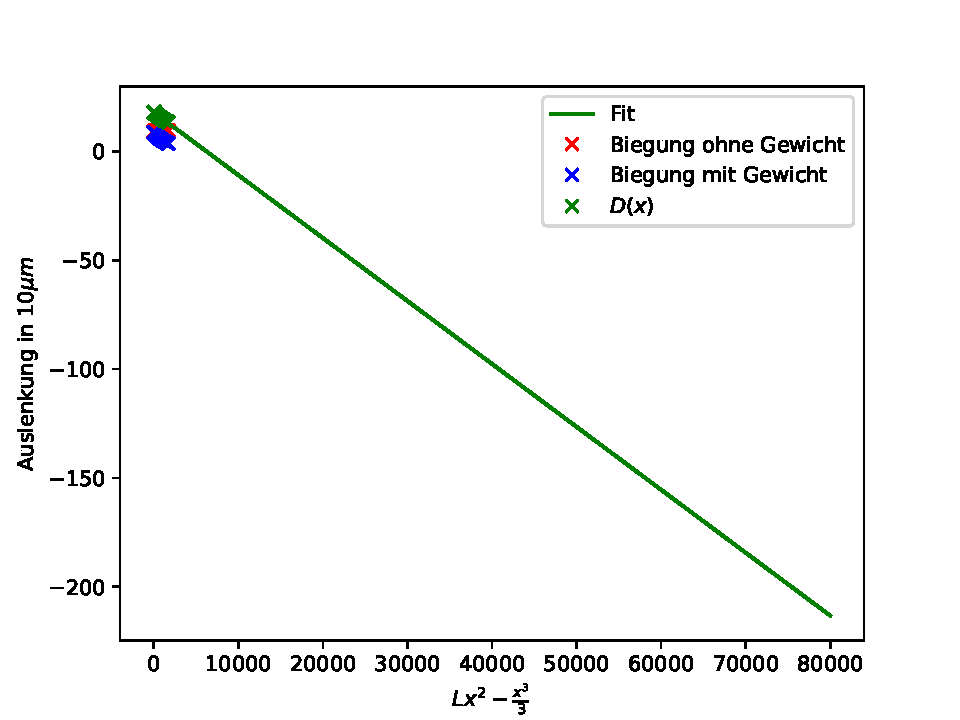
\includegraphics{build/plot1.pdf}
  \caption{Eckiger Stab, einseitige Einspannung}
  \label{fig:plot1}
\end{figure}

Über die Differenz der Auslenkung  ergibt sich nach
$D(x) = D_0 - D_m$(Tab.2). Die Einspannlänge beträgt $L_1 = 0.493m$ und
das verwendete Gewicht wiegt $m_1 = 1.1932 kg$.





Mit Hilfe von Python wird eine Regressiongerade berechnet (Abb.3).
Hierbei wird $(Lx^2- \frac{x^3}{3})$ auf der x-Achse gegen $D(x)$ auf der y-Achse
gesetzt, woraus sich die Werte
\begin{align*}
  a &= \SI{7.8205(257)e-2}{\per\square\meter} \\
  %b &= \SI{8.15(104)e-5}{\meter} \\
\end{align*}
für die Regressionsgerade ergeben.
\newline
Das vorliegende Flächenträgheitsmoment ist nach (\ref{eqn:Iquadrat})
\begin{equation*}
  I = 8.333 * 10^{-10}\, m^4.
\end{equation*}

Hiermit wird der Elastizitätsmodul nach (\ref{eqn:einseitig}) bestimmt.

\begin{equation*}
  E = \SI{88.01(33)e9}{\newton\per\square\meter}
\end{equation*}
\newpage






\subsection{Runder Stab, einseitige Einspannung}
Die Einspannlänge beträgt nun $L_2 = 0.508m$, es wird ein Gewicht
mit $m_2 = 0.5339 kg $ verwendet und die Aulenkungen $D(x)$ finden
sich in Tabelle.4.

\begin{table}[h]
  \centering
  \label{tab:4}
  \begin{tabular}{ c c }
    \toprule
    $x \,\, \text{in} \, [mm]$
   &{$D(x) \,\, \text{in} \, [mm]$} \\
   %&{$(Lx^2- \frac{x^3}{3}) \,\, \text{in} \, [10^{-3}m^3]$} \\

    \midrule
    30 & 0.030 \\% 0.45\\
    50 & 0.110 \\% 1.23\\
    70 & 0.175 \\% 2.38\\
    90 & 0.255 \\% 3.87\\
    110& 0.400 \\% 5.70\\
    130& 0.540 \\% 7.85\\
    150& 0.700 \\%10.31\\
    170& 0.870 \\%13.04\\
    190& 1.070 \\%16.05\\
    210& 1.285 \\%19.32\\
    230& 1.495 \\%22.82\\
    250& 1.715 \\%26.54\\
    270& 1.970 \\%30.47\\
    290& 2.280 \\%34.59\\
    310& 2.525 \\%38.89\\
    330& 2.815 \\%43.34\\
    350& 3.030 \\%47.94\\
    370& 3.305 \\%52.66\\
    390& 3.730 \\%57.49\\
    410& 4.050 \\%62.42\\
    430& 4.165 \\%67.43\\
    450& 4.560 \\%72.50\\
    470& 4.900 \\%77.61\\
    490& 5.090 \\%82.75\\

    \bottomrule
  \end{tabular}
  \caption{Auslenkung runder Stab.}
\end{table}

\begin{figure}[h]
  \centering
  \includegraphics{build/plot2.pdf}
  \caption{Runder Stab, einseitige Einspannung.}
  \label{fig:plot2}
\end{figure}

Die erneute Berechnung des Regressionsgeraden(Abb.4) über Python
für die vorliegenden Werte ergibt
\begin{align*}
  a &= \SI{6.2320(417)e-2}{\per\square\meter} \\
  %b &= \SI{5.64(176)e-5}{\meter} \\
\end{align*}
und das Flächenträgheitsmoment lautet nach (\ref{eqn:Ikreis})
\begin{equation}
  I = 4.909* 10^{-10} m^4.
  \label{const:Ikreis}
\end{equation}
\newline
Wodurch sich für den Elastizitätsmodul mit (\ref{eqn:einseitig})
\begin{equation*}
  E = \SI{84.18(40)e9}{\newton\per\square\meter}
\end{equation*}
ergibt.
\newpage
\subsection{Runder Stab, beidseitige Einspannung, rechts}
Aufgrund des unterschiedlichen Biegeverhaltens wird nun $(3L^2x-4x^3)$
auf der x-Achse verwendet. Die Einspannlänge beträgt $L_3 = 0.565m$
und es wird ein Gewicht mit $m_3 = 4.6937 kg$ genutzt.

\begin{table}[h]
  \centering
  \label{tab:5}
  \begin{tabular}{ c c }
    \toprule
    $x \,\, \text{in} \, [mm]$
   &{$D(x) \,\, \text{in} \, [mm]$}\\
   %&{$(3L^2x-4x^3)\,\, \text{in} \, [10^{-3}m^3]$} \\

    \midrule
    30  & 0.110 \\%28.62\\
    50  & 0.155 \\%47.38\\
    70  & 0.270 \\%65.67\\
    90  & 0.410 \\%83.27\\
    110 & 0.540 \\%100.02\\
    130 & 0.730 \\%115.71\\
    150 & 0.920 \\%130.15\\
    170 & 1.105 \\%143.15\\
    190 & 1.255 \\%154.52\\
    210 & 1.425 \\%164.06\\
    230 & 1.535 \\%171.59\\
    250 & 1.645 \\%176.91\\
    270 & 1.745 \\%179.84\\

    \bottomrule
  \end{tabular}
  \caption{Auslenkung runder Stab, rechts.}
\end{table}

\begin{figure}
  \centering
  \includegraphics{build/plot3.pdf}
  \caption{Runder Stab, beidseitige Einspannung, rechts.}
  \label{fig:plot3}
\end{figure}
Für die Regressionsgerade(Abb.5) ergeben sich:
\begin{align*}
  a &= \SI{1.1156(67)e-2}{\per\square\meter} \\
  %b &= \SI{-4.28(87)e-4}{\meter} \\
\end{align*}
Zusammen mit dem Flächenträgheitsmoment aus (\ref{const:Ikreis})
%\begin{equation*}
%  I = 9.818*10^{-10}\, m^4.
%\end{equation*}
ergibt sich für den Elastizitätsmodul mit (\ref{eqn:beidseitigr})
\begin{equation*}
  E = \SI{241.17(1299)e9}{\newton\per\square\meter} .
\end{equation*}
\newpage

\subsection{Runder Stab, beidseitige Einspannung, links}
Aufgrund des unterschiedlichen Biegeverhaltens wird nun $\left(4x^3-12Lx^2+9L^2x-L^3\right)$
auf der x-Achse verwendet. Die Einspannlänge beträgt $L_3 = 0.565m$
und es wird ein Gewicht mit $m_3 = 4.6937 kg$ genutzt.

\begin{table}[h]
  \centering
  \label{tab:lit5}
  \begin{tabular}{ c c  }
    \toprule
    $x \,\, \text{in} \, [mm]$
   &{$D(x) \,\, \text{in} \, [mm]$}\\
   %&{$(3L^2x-4x^3)\,\, \text{in} \, [10^{-3}m^3]$} \\

    \midrule
    290 & 1.765 \\
    310 & 1.770 \\
    330 & 1.805 \\
    350 & 1.720 \\
    370 & 1.650 \\
    390 & 1.570 \\
    410 & 1.370 \\
    430 & 1.225 \\
    450 & 1.090 \\
    470 & 0.930 \\
    490 & 0.735 \\
    510 & 0.585 \\
    530 & 0.280 \\
    550 & 0.070 \\


    \bottomrule
  \end{tabular}
  \caption{Auslenkung runder Stab, links.}
\end{table}

\begin{figure}
  \centering
  \includegraphics{build/plot4.pdf}
  \caption{Runder Stab, beidseitige Einspannung, links.}
  \label{fig:plot4}
\end{figure}
Für die Regressionsgerade(Abb.6) ergeben sich:
\begin{align*}
  a &= \SI{1.028(1)e-2}{\per\square\meter} \\
  %b &= \SI{-4.28(87)e-4}{\meter} \\
\end{align*}
Zusammen mit dem Flächenträgheitsmoment aus (\ref{const:Ikreis})
%\begin{equation*}
%  I = 9.818*10^{-10}\, m^4.
%\end{equation*}
ergibt sich für den Elastizitätsmodul mit (\ref{eqn:beidseitigl})
\begin{equation*}
  E = \SI{190.10(191)e9}{\newton\per\square\meter} .
\end{equation*}
\newpage
